\documentclass[a4paper, 12pt]{report}
\usepackage{graphicx}
\usepackage[utf8]{inputenc}
\usepackage[ngerman]{babel}
\usepackage{geometry}
\usepackage{csquotes}
\usepackage[toc,page]{appendix}
\usepackage{titlesec}
\usepackage{listings}
\usepackage{float}
\usepackage[hang,flushmargin]{footmisc} 
\usepackage{makecell}
\usepackage{amsmath}% http://ctan.org/pkg/amsmath
\usepackage[utf8]{inputenc}
\usepackage[default]{cantarell} %% Use option "defaultsans" to use cantarell as sans serif only
\usepackage[T1]{fontenc}
\usepackage{hyperref}
\usepackage{helvet}
\usepackage[eulergreek]{sansmath}
\usepackage{amsfonts}
\usepackage{movie15}
\usepackage{url}

\usepackage{tikz}
\usetikzlibrary{calc,positioning,shapes,decorations.pathreplacing}
\usetikzlibrary{fit,fadings,shadows,patterns,math}
\usetikzlibrary{shapes.arrows,shapes.geometric}
\usetikzlibrary{arrows,arrows.meta,decorations.markings}
\usetikzlibrary{decorations.pathmorphing}

\usepackage{pgfplots}

\graphicspath{ {./images/} }
\geometry{margin=1.25in}

\newcommand*{\shifttext}[2]{%
  \settowidth{\@tempdima}{#2}%
  \makebox[\@tempdima]{\hspace*{#1}#2}%
}
\newcommand{\fakesection}[1]{%
  \par\refstepcounter{section}% Increase section counter
  \sectionmark{#1}% Add section mark (header)
  \addcontentsline{toc}{section}{\protect\numberline{\thesection}#1}% Add section to ToC
  % Add more content here, if needed.
}
\titleformat{\chapter}[display]
  {\normalfont\bfseries}{}{0pt}{\Large}
\titleformat*{\section}{\large\bfseries}

\renewcommand{\footnoterule}{%
  \kern -3pt
  \hrule width \textwidth height 1pt
  \kern 2pt
}

\newcommand\blfootnote[1]{%
  \begingroup
  \renewcommand\thefootnote{}\footnote{#1}%
  \addtocounter{footnote}{-1}%
  \endgroup
}

\begin{document}

\begin{center}
    \vspace*{2em}
    \normalsize 1. Projekt\\
    \vspace*{1em}
    \normalsize \textbf{\textit{Ableitungsfreie Methoden}}\\
    \vspace*{4em}
    \normalsize im Fach\\
    \vspace*{1em}
    \large Numerische Optimierung\\
    \vspace*{30em}
    \normalsize Mai 2020\\
    \vspace*{1em}
    \normalsize Maximilian Gaul
\end{center}

\thispagestyle{empty}

\newpage

\subsubsection{Aufgabe 1}
Teilintervalle und Funktionswerte des Bisektionsverfahrens aus \lstinline[basicstyle=\ttfamily\color{black}]|Bisektion.m|
für das Minimum von
$$h(x) = e^{-x} + 0.5x^2$$
mit dem Startintervall [0, 1] nach 10 Schritten:
\begin{figure}[H]
  \centering
  \def\arraystretch{1.25}
  \begin{tabular}{l|c|r}
    \hline
    \textbf{Schritt} & \textbf{Intervall} & \makecell{\textbf{Funktionswert}}\\
    \hline
    1 & [0.00, 1.00] & h(0.50)=0.7315\\
    2 & [0.50, 1.00] & h(0.75)=0.7536\\
    3 & [0.50, 0.75] & h(0.63)=0.7306\\
    4 & [0.50, 0.63] & h(0.56)=0.7280\\
    5 & [0.56, 0.63] & h(0.59)=0.7285\\
    6 & [0.56, 0.59] & h(0.58)=0.7281\\
    7 & [0.56, 0.58] & h(0.57)=0.7280\\
    8 & [0.56, 0.57] & h(0.57)=0.7280\\
    9 & [0.57, 0.57] & h(0.57)=0.7280\\
    10 & [0.57, 0.57] & h(0.57)=0.7280\\
    \hline
  \end{tabular}
  \caption{Die ersten 10 Schritte des Bisektionsverfahrens mit Startintervall [0, 1] für $h(x)$}
\end{figure}
Die Intervallgrenzen und Funktionsauswertungen sind wie folgt verteilt:
\begin{figure}[H]
  \centering
  \begin{tikzpicture}
    \newcommand*{\scaleFactor}{4}
    \tikzstyle{interval border}=[thin, red];

    \draw[-{Latex}] (-0.5,0) -- (1.25*\scaleFactor,0) node[right] {$x$};
    \draw[-{Latex}] (0,-0.5) -- (0,1.25*\scaleFactor) node[above] {$h(x)$};
    \draw[scale=\scaleFactor, thick, black, domain=-0.25:1.25, smooth, variable=\x] plot ({\x},{exp(-\x) + 0.5*\x^2});

    \foreach \i in {0, 0.50, 0.75, 0.625, 0.5625, 0.5664, 0.5938, 0.5781, 0.5703, 0.5684, 1} {
      \draw[interval border] (\i*\scaleFactor, 0) -- (\i*\scaleFactor, 1.25*\scaleFactor);
    }

    \foreach \x / \y / \i in {0.5/0.7315/1, 0.75/0.7536/2, 0.625/0.7306/3, 0.5625/0.7280/4, 0.5938/0.7285/5, 0.5781/0.7281} {
      \draw (\x*\scaleFactor, \y*\scaleFactor) node[interval border] {x};
    }
  \end{tikzpicture}
  \caption{$h(x)$ mit Intervallgrenzen und Auswertungspunkten des Bisektionsverfahrens}
\end{figure}

\subsubsection{Aufgabe 2}
Siehe \lstinline[basicstyle=\ttfamily\color{black}]|Mutation.m|.

\subsubsection{Aufgabe 3}
Nachfolgende Erläuterungen beziehen sich auf 
$$f(x_1, x_2) = (x_1^2 + x_2 - 11)^2 + (x_1 + x_2^2 - 7)^2 \text{ mit Startwert } f_0=\begin{bmatrix}2\\4\end{bmatrix}$$
$$g(x_1, x_2) = 100\cdot (x_1 - 2)^4 + (x_1 - 2x_2)^2 \text{ mit Startwert } g_0=\begin{bmatrix}4\\2\end{bmatrix}$$
Eine Möglichkeit für ein Abbruchkriterium ist die Anzahl an Iterationen, d.h. der Algorithmus stoppt nach einer bestimmten Anzahl an Durchläufen
und gibt den bis dahin berechneten Wert aus. Je nach Funktion und Zufallsvektoren kann die Genauigkeit des Ergebnisses stark schwanken. Während für
eine festgelegte obere Grenze an Durchläufen für eine simple Funktion ein Minimum bereits ausreichend genau bestimmt werden kann, benötigt eine
komplexere Funktion ggf. weitaus mehr Durchläufe. Die Anzahl an Iterationen ist also kein adaptives Kriterium.\par
Weiterhin könnte auch der Betrag aus der Differenz des aktuellen Funktionswertes und des letzten Funktionswertes als Abbruchkriterium funktionieren.
Dabei aktualisiert man die zu überprüfenden Werte nur, sofern eine Verbesserung eingetreten ist (ansonsten wären letzter und aktueller Funktionswert
eventuell gleich). Ist der Differenzbetrag kleiner als eine festgelegte Toleranz, endet der Algorithmus. Typische Werte sind hier z.B. $10^{-4}$ oder
$10^{-8}$.\\\par

\begin{figure}[H]
  \centering
  \def\arraystretch{1.25}
  \begin{tabular}{l|c|c|r}
    \hline
    \textbf{Kriterium} & \textbf{Funktion} & \textbf{Genauigkeit} & \textbf{Anzahl Schritte}\\
    \hline
    Differenzbetrag & f & $10^{-6}$ & 4.924.700\\
    Differenzbetrag & f & $10^{-6}$ & 282.179\\
    Differenzbetrag & f & $10^{-6}$ & 24.907\\
    Differenzbetrag & g & $10^{-6}$ & 36.655\\
    Differenzbetrag & g & $10^{-6}$ & 9.758\\
    Differenzbetrag & g & $10^{-6}$ & 882\\
    \hline
  \end{tabular}
  \caption{Einfluss des Zufalls auf die Anzahl an Durchläufen für eine Genauigkeit von $10^{-6}$ bei festem $\alpha$}
  \label{fig:mutSelTbl}
\end{figure}

Durch die Wahl des Differenzbetrages kann man vom Zufall profitieren und mit verhältnismäßig wenigen Schritten zu einer guten Genauigkeit kommen.
Wählt man dagegen die Anzahl der Iterationen, muss man ggf. neu rechnen wenn das Ergebnis noch zu ungenau ist:

\begin{figure}[H]
  \centering
  \def\arraystretch{1.25}
  \begin{tabular}{l|c|c|r}
    \hline
    \textbf{Abbruchkriterium} & \textbf{Funktion} & \textbf{Genauigkeit} & \textbf{Anzahl Schritte}\\
    \hline
    Anzahl Iterationen & f & $1\cdot 10^{-5}$ & 225.000\\
    Anzahl Iterationen & f & $7\cdot 10^{-6}$ & 225.000\\
    Anzahl Iterationen & f & $2\cdot 10^{-8}$ & 225.000\\
    Anzahl Iterationen & g & $2\cdot 10^{-6}$ & 15.000\\
    Anzahl Iterationen & g & $6\cdot 10^{-7}$ & 15.000\\
    Anzahl Iterationen & g & $1\cdot 10^{-8}$ & 15.000\\
    \hline
  \end{tabular}
  \caption{Einfluss des Zufalls auf die Genauigkeit bei einer gegebenen Anzahl an Durchläufen bei festem $\alpha$}
\end{figure}

Der Parameter $\alpha$ bestimmt den Anteil des Zufallsvektors für den Wert von $\hat x$. Kleine Werte von $\alpha$ bedeuten eine höhere Wahrscheinlichkeit,
dass sich der Funktionswert verbessert (die Verbesserung fällt aber möglicherweise kleiner aus) da sich besonders in der Nähe eines Minimums,
bei quadratischen oder Funktionen 4. Grades der Funktionswert stark ändern und man leicht über das Ziel hinaus schießen kann wenn man zu große
Schritte geht (ähnlich wie bei einem Abstiegsverfahren). Falls die Ableitung der Funktion zur Verfügung steht (tut sie hier wahrscheinlich nicht da
das Projekt \textit{Ableitungsfreie Methoden} heißt), könnte man ein Verfahren zur Schrittweitensteuerung implementieren
(z.B. nach Armijo $\varphi(\alpha) := f(x + \alpha r)$).\par

\begin{figure}[H]
  \centering
  \def\arraystretch{1.25}
  \begin{tabular}{l|c|c|r|r}
    \hline
    \textbf{Abbruchkriterium} & \textbf{Funktion} & \textbf{Genauigkeit} & $\overline{ \text{\textbf{Anzahl Schritte}} }_{200}$ & \textbf{$\alpha$}\\
    \hline
    Differenzbetrag & f & $10^{-4} $ & 238.992 & 1\\
    Differenzbetrag & f & $10^{-4} $ & 190.980 & 0.5\\
    Differenzbetrag & f & $10^{-4} $ & 19.557 & 0.25\\
    Differenzbetrag & f & $10^{-4} $ & 9.025 & 0.125\\
    Differenzbetrag & g & $10^{-4} $ & 41.688 & 1\\
    Differenzbetrag & g & $10^{-4} $ & 1.878 & 0.5\\
    Differenzbetrag & g & $10^{-4} $ & 1.101 & 0.25\\
    Differenzbetrag & g & $10^{-4} $ & 383 & 0.125\\
    \hline
  \end{tabular}
  \caption{Einfluss von $\alpha$ auf den Durchschnitt von 200 Durchläufen für eine Genauigkeit von $10^{-4}$}
\end{figure}

Zu Beginn von \lstinline[basicstyle=\ttfamily\color{black}]|Mutation-Selektion| sind die Sprünge der Funktionswerte relativ groß, werden dann aber
immer kleiner:

\begin{figure}[H]
  \centering
  \def\arraystretch{1.25}
  \begin{tabular}{l|c|r}
    \hline
    \textbf{Funktion} & \textbf{x} & \textbf{Funktionswert}\\
    \hline
    f & [2.10 3.82] & 101.61\\
    f & [1.85 3.60] & 76.25\\
    f & [2.11 3.55] & 68.41\\
    f & [2.29 3.37] & 50.06\\
    f & [2.02 3.03] & 32.96\\
    f & [2.39 2.68] & 13.39\\
    f & [2.41 2.24] & 9.01\\
    f & [2.42 2.39] & 8.99\\
    f & [2.71 2.37] & 3.44\\
    f & [2.81 2.32] & 2.03\\
    f & [3.20 1.88] & 1.35\\
    f & [3.09 2.12] & 0.80\\
    f & [2.98 1.79] & 0.77\\
    \hline
  \end{tabular}
  \caption{Die ersten Schritte eines Aufrufes von \lstinline[basicstyle=\ttfamily\color{black}]|Mutation-Selektion| mit $\alpha = 1$}
\end{figure}

Eine Strategie könnte daher sein, $\alpha$ erst klein zu wählen (z.B. 0.125) und dann mit jeder Iteration zu vergrößern dabei aber
nicht über eine obere Schranke zu kommen (z.B. 0.5). Dies geschieht unter der Annahme, das der Algorithmus zuerst die richtige
Richtung finden muss, durch zu große Sprünge werden diese im ungünstigen Fall verpasst d.h. man geht zu weit in eine Richtung.

\begin{figure}[H]
  \centering
  \def\arraystretch{1.25}
  \begin{tabular}{l|c|r|r|r}
    \hline
    \textbf{Funktion} & \textbf{Genauigkeit} & $\overline{ \text{\textbf{Anzahl Schritte}} }_{600}$ & \textbf{$\alpha$} & \textbf{Verstärkungsfaktor}\\
    \hline
    f & $10^{-4}$ & 5.062 & 0.1250 & 1.1000\\
    f & $10^{-4}$ & 3.660 & 0.1250 & 1.0500\\
    f & $10^{-4}$ & 3.850 & 0.1250 & 1.0250\\
    f & $10^{-4}$ & 6.639 & 0.1250 & 1.0125\\
    g & $10^{-4}$ & 438 & 0.1250 & 1.1000\\
    g & $10^{-4}$ & 386 & 0.1250 & 1.0500\\
    g & $10^{-4}$ & 368 & 0.1250 & 1.0250\\
    g & $10^{-4}$ & 771 & 0.1250 & 1.0125\\
    \hline
  \end{tabular}
  \caption{Einfluss von $\alpha$ und einem Verstärkungsfaktor auf den Durchschnitt an Iterationen für eine Genauigkeit von $10^{-4}$}
\end{figure}

Man sieht, dass durch einen Verstärkungsfaktor zwischen in [1.025, 1.05] die Anzahl an Iterationen reduziert werden konnte. Wird der
Faktor zu klein gewählt (d.h. $\alpha$ bleibt über einen großen Teil des Durchlaufs relativ klein) verlängert sich die Rechenzeit wieder.

\begin{figure}[H]
  \centering
  \begin{minipage}[t]{.32\textwidth}
    \begin{tikzpicture}[scale=0.625]
      \begin{axis}[
        view={60}{30}
      ]
      \addplot3[
        surf, fill opacity=.5, domain=1:5, ylabel={y}, xlabel={x}, zlabel={f(x,y)}, width=3cm, height=3cm, samples=32] { (x^2 + y - 11)^2 + (x + y^2 - 7)^2 };
      \addplot3[
        only marks, mark size=2pt, mark=*, mark options={fill=red, draw=black}, width=3cm, height=3cm
      ] table [x=X, y=Y, z=Z, col sep=comma] {
              X,        Y,      Z
              1.9962,	3.9797,	126.5975
              2.0165,	3.9396,	119.9972
              1.9886,	3.9246,	117.7146
              2.0161,	3.9227,	117.3179
              2.0782,	3.9143,	115.8161
              2.0998,	3.8748,	109.6665
              2.1104,	3.8286,	102.8133
              2.1241,	3.8061,	99.5540
              2.1679,	3.7476,	91.3898
              2.2175,	3.7487,	91.3844
              2.2501,	3.6908,	83.7619
              2.3047,	3.6740,	81.5544
              2.2658,	3.6516,	78.8693
              2.3076,	3.6449,	77.9592
              2.3043,	3.6237,	75.4260
              2.3438,	3.5867,	71.0592
              2.3771,	3.5521,	67.1479
              2.3483,	3.5281,	64.6071
              2.3376,	3.5084,	62.5815
              2.3436,	3.4572,	57.4344
              2.3936,	3.3957,	51.4649
              2.4100,	3.3605,	48.2831
              2.4614,	3.3461,	46.8720
              2.4078,	3.3084,	43.9546
              2.4688,	3.2985,	42.8897
              2.4544,	3.2402,	38.4573
              2.4883,	3.1931,	34.9163
              2.4903,	3.1685,	33.2345
              2.4530,	3.1310,	31.0579
              2.4217,	3.0763,	28.1042
              2.4259,	3.0617,	27.2562
              2.4773,	3.0426,	25.7303
              2.4713,	2.9903,	23.0953
              2.5291,	2.9370,	20.0416
              2.5279,	2.9083,	18.7824
              2.5639,	2.8659,	16.7010
              2.6043,	2.8204,	14.6171
              2.6159,	2.8156,	14.3551
              2.6708,	2.8220,	14.3002
              2.6114,	2.7717,	12.8340
              2.6318,	2.7353,	11.4847
              2.5976,	2.6977,	10.6842
              2.6027,	2.6486,	9.3398
              2.6421,	2.6462,	8.8782
              2.6755,	2.6463,	8.6036
              2.6917,	2.6041,	7.4391
              2.7457,	2.5897,	6.7727
              2.6992,	2.5455,	6.1122
              2.6755,	2.4993,	5.4966
              2.7360,	2.4494,	4.1463
              2.7479,	2.3955,	3.3189
              2.7976,	2.3880,	2.8682
              2.7970,	2.3376,	2.2960
              2.7895,	2.3119,	2.1095
              2.7756,	2.2532,	1.8149
              2.8038,	2.1911,	1.2639
              2.8271,	2.2118,	1.1504
              2.8692,	2.1592,	0.6523
              2.9173,	2.1801,	0.5448
              2.9574,	2.1337,	0.2746
              2.9645,	2.0860,	0.1156
              3.0046,	2.0341,	0.0240
              3.0146,	2.0037,	0.0093
              3.0058,	1.9757,	0.0084
              2.9888,	1.9945,	0.0063
              3.0002,	1.9945,	0.0005
              3.0036,	1.9993,	0.0004
              3.0028,	1.9960,	0.0003
              2.9985,	2.0040,	0.0002
              3.0018,	2.0011,	0.0002
              3.0003,	2.0017,	0.0001
              2.9988,	2.0003,	0.0000
        };
      \end{axis}
    \end{tikzpicture}
    \caption{$\alpha = 0.125$ mit Verstärkungsfaktor 1.05}
  \end{minipage}
  \begin{minipage}[t]{.32\textwidth}
    \begin{tikzpicture}[scale=0.625]
      \begin{axis}[
        view={60}{30}
      ]
      \addplot3[
        surf, fill opacity=.5, domain=1:5, ylabel={y}, xlabel={x}, zlabel={f(x,y)}, width=3cm, height=3cm, samples=32] { (x^2 + y - 11)^2 + (x + y^2 - 7)^2 };
      \addplot3[
        only marks, mark size=2pt, mark=*, mark options={fill=red, draw=black}, width=3cm, height=3cm
      ] table [x=X, y=Y, z=Z, col sep=comma] {
              X,        Y,      Z
              1.9476,	3.9652,	124.3630
              1.9074,	3.9232,	117.8902
              1.9366,	3.8890,	112.5093
              1.9511,	3.8531,	107.1493
              1.9229,	3.8000,	99.9345
              1.8991,	3.7517,	93.8061
              1.9576,	3.6905,	85.6639
              1.9849,	3.6666,	82.5625
              1.9255,	3.6574,	82.1334
              1.9037,	3.6260,	78.8931
              1.8749,	3.6222,	78.8384
              1.8362,	3.6130,	78.3791
              1.7972,	3.5866,	76.1913
              1.8083,	3.5555,	72.9293
              1.7984,	3.5407,	71.6523
              1.7767,	3.4852,	66.9246
              1.7180,	3.4505,	65.0187
              1.7209,	3.4268,	63.0516
              1.7484,	3.3720,	58.3314
              1.7297,	3.3369,	56.2154
              1.7242,	3.2771,	52.4156
              1.7736,	3.2235,	48.1180
              1.7176,	3.1912,	47.6291
              1.7564,	3.1363,	43.9298
              1.7657,	3.0759,	40.9663
              1.8015,	3.0651,	39.5982
              1.8153,	3.0122,	37.1410
              1.7729,	2.9578,	36.4013
              1.8118,	2.9509,	35.1072
              1.8477,	2.8981,	32.5179
              1.9003,	2.8727,	30.3370
              1.9602,	2.8280,	27.4954
              2.0213,	2.8635,	26.7855
              2.0671,	2.8447,	25.0552
              2.0540,	2.8183,	24.6835
              2.0874,	2.8434,	24.4976
              2.1089,	2.8149,	23.1672
              2.1490,	2.7931,	21.5849
              2.1897,	2.8138,	21.1556
              2.2374,	2.7834,	19.2151
              2.2770,	2.7721,	18.0326
              2.2824,	2.7399,	17.0867
              2.2605,	2.7154,	17.0170
              2.2715,	2.6692,	15.7963
              2.3142,	2.6126,	13.7715
              2.3246,	2.5633,	12.7897
              2.3097,	2.5017,	12.4667
              2.3653,	2.4679,	10.7492
              2.4145,	2.4762,	9.6492
              2.4496,	2.4445,	8.5597
              2.4815,	2.4000,	7.5053
              2.5238,	2.4122,	6.7238
              2.5498,	2.3565,	5.8041
              2.5691,	2.3462,	5.3695
              2.5841,	2.2846,	4.7982
              2.6287,	2.2933,	4.0161
              2.6718,	2.3525,	3.7310
              2.6786,	2.2939,	3.2293
              2.6786,	2.2872,	3.1930
              2.7051,	2.2353,	2.5862
              2.7042,	2.1771,	2.4784
              2.7280,	2.1273,	2.1107
              2.7762,	2.1137,	1.4502
              2.8068,	2.0974,	1.0915
              2.8265,	2.1000,	0.8860
              2.8737,	2.0470,	0.4867
              2.8988,	2.0608,	0.3085
              2.9096,	2.0023,	0.2894
              2.9230,	2.0376,	0.1807
              2.9461,	2.0203,	0.0910
              3.0037,	1.9835,	0.0039
              3.0006,	2.0033,	0.0002
              3.0012,	1.9982,	0.0001
              2.9990,	2.0016,	0.0000
              2.9992,	2.0002,	0.0000
              3.0002,	1.9995,	0.0000
              3.0000,	2.0002,	0.0000
              2.9999,	2.0001,	0.0000
        };
      \end{axis}
    \end{tikzpicture}
    \caption{$\alpha = 0.125$}
  \end{minipage}
  \begin{minipage}[t]{.32\textwidth}
    \begin{tikzpicture}[scale=0.625]
      \begin{axis}[
        view={60}{30}
      ]
      \addplot3[
        surf, fill opacity=.5, domain=1:5, ylabel={y}, xlabel={x}, zlabel={f(x,y)}, width=3cm, height=3cm, samples=32] { (x^2 + y - 11)^2 + (x + y^2 - 7)^2 };
      \addplot3[
        only marks, mark size=2pt, mark=*, mark options={fill=red, draw=black}, width=3cm, height=3cm
      ] table [x=X, y=Y, z=Z, col sep=comma] {
              X,        Y,      Z
              2.0223,	3.8754,	110.0305
              2.0347,	3.7935,	98.2342
              1.9145,	3.7449,	92.7908
              1.9231,	3.6246,	78.4957
              1.8372,	3.5160,	68.7165
              1.9499,	3.4270,	59.0305
              1.8341,	3.3388,	54.2491
              1.8991,	3.3201,	51.6653
              1.9631,	3.3162,	50.1952
              1.9328,	3.2500,	46.3145
              1.9088,	3.1464,	40.8473
              1.8180,	3.0564,	38.8152
              1.8797,	2.9833,	34.3898
              1.9183,	2.9613,	32.5975
              2.0387,	2.9774,	30.1850
              2.1601,	2.8679,	23.4733
              2.0926,	2.7569,	22.1838
              2.1484,	2.6368,	18.4581
              2.1368,	2.5673,	17.9360
              2.2224,	2.6470,	16.6229
              2.2987,	2.5729,	13.5587
              2.4181,	2.5374,	10.2874
              2.4549,	2.5621,	9.8915
              2.4563,	2.4873,	8.8465
              2.5142,	2.4601,	7.3754
              2.6268,	2.3639,	4.4895
              2.7319,	2.4052,	3.5810
              2.7439,	2.3114,	2.5252
              2.8555,	2.3297,	1.9130
              2.9589,	2.2664,	1.2010
              2.9360,	2.1866,	0.5518
              2.8852,	2.0842,	0.4024
              2.9456,	2.0627,	0.1080
              3.0077,	2.0270,	0.0189
              3.0027,	2.0024,	0.0005
              3.0005,	2.0011,	0.0000
              2.9996,	2.0006,	0.0000
              3.0003,	2.0000,	0.0000
              3.0001,	2.0000,	0.0000
              3.0000,	2.0002,	0.0000
        };
      \end{axis}
    \end{tikzpicture}
    \caption{$\alpha = 0.25$}
  \end{minipage}
\end{figure}

\subsubsection{Aufgabe 4}
Vergleich der Rechenzeit für die Funktionen $f, g, h$ mit dem Bisektions- und Mutation-Selektion-Verfahren sowie
\lstinline[basicstyle=\ttfamily\color{black}]|fminsearch|. Da das Bisektionsverfahren nur im eindimensionalen Fall funktioniert
wird es nur auf $h$ angewendet.

\begin{figure}[H]
  \centering
  \pgfplotstableread{
    0 0.024631  0.909518      0.544333
  }\dataseth
  \pgfplotstableread{
    0 0.0       1212.082227   1.254401
  }\datasetf
  \pgfplotstableread{
    0 0.0       16.337017     3.398372
  }\datasetg
  \begin{minipage}{.3\textwidth}
    \begin{tikzpicture}
        \begin{axis}[
            width=4cm,
            height=6.5cm,
            ybar,
            ymin=0,
            ylabel={Rechenzeit in ms},
            ytick=\empty,
            extra y ticks={0,0.25,0.5,0.75,1.0,1.25},
            extra y tick labels={{0},{0.25},{0.5},{0.75},{1.0},{1.25}},
            xtick=data,
            xticklabels={
                h(x)
            },
            xticklabel style={yshift=-12ex},
            major x tick style={
                % (this is a better way than assigning `opacity=0')
                /pgfplots/major tick length=0pt,
            },
            minor x tick num=1,
            minor tick length=2ex,
            % ---------------------------------------------------------------------
            % (adapted solution from <https://tex.stackexchange.com/a/141006/95441>)
            % we want to provide absolute `at' values ...
            scatter/position=absolute,
            node near coords style={
                % ... to provide axis coordinates at `ymin' for the nodes
                at={(axis cs:\pgfkeysvalueof{/data point/x},\pgfkeysvalueof{/pgfplots/ymin})},
                % then also the `anchor' has to be adapted ...
                anchor=east,
                % ... because we rotate the labels which would overlap otherwise
                rotate=90,
            },
            % ---------------------------------------------------------------------
            % (created a cycle list to shorten the below `\addplot' entries)
            cycle list={
                {draw=black,fill=black!20},
                {draw=black,fill=black!40},
                {draw=black,fill=black!60},
            },
            % (moved common option here)
            table/x index=0,
        ]
            \addplot+ [nodes near coords=Bisekt.] table [y index=1] \dataseth;
            \addplot+ [nodes near coords=Mut.-Selekt.] table [y index=2] \dataseth;
            \addplot+ [nodes near coords=fminsearch] table [y index=3] \dataseth;
        \end{axis}
        \node[black, rotate=90] (impl) at (0.79,1.025) {0.025};
        \draw[-{Latex}, thick, black] (impl.west) -- ([yshift=-0.2cm]impl.west);
    \end{tikzpicture}
  \end{minipage}
  \begin{minipage}{.3\textwidth}
    \begin{tikzpicture}
        \begin{axis}[
            width=4cm,
            height=6.5cm,
            ybar,
            ymin=0,
            ytick=\empty,
            extra y ticks={0,250,500,750,1000,1250},
            extra y tick labels={{0},{250},{500},{750},{1000},{1250}},
            xtick=data,
            xticklabels={
                f(x)
            },
            xticklabel style={yshift=-12ex},
            major x tick style={
                % (this is a better way than assigning `opacity=0')
                /pgfplots/major tick length=0pt,
            },
            minor x tick num=1,
            minor tick length=2ex,
            % ---------------------------------------------------------------------
            % (adapted solution from <https://tex.stackexchange.com/a/141006/95441>)
            % we want to provide absolute `at' values ...
            scatter/position=absolute,
            node near coords style={
                % ... to provide axis coordinates at `ymin' for the nodes
                at={(axis cs:\pgfkeysvalueof{/data point/x},\pgfkeysvalueof{/pgfplots/ymin})},
                % then also the `anchor' has to be adapted ...
                anchor=east,
                % ... because we rotate the labels which would overlap otherwise
                rotate=90,
            },
            % ---------------------------------------------------------------------
            % (created a cycle list to shorten the below `\addplot' entries)
            cycle list={
                {draw=black,fill=black!40},
                {draw=black,fill=black!60},
            },
            % (moved common option here)
            table/x index=0,
        ]
            \addplot+ [nodes near coords=Mut.-Selekt.] table [y index=2] \datasetf;
            \addplot+ [nodes near coords=fminsearch] table [y index=3] \datasetf;
        \end{axis}
        \node[black, rotate=90] (impl) at (1.425,0.8) {1.25};
        \draw[-{Latex}, thick, black] (impl.west) -- ([yshift=-0.2cm]impl.west);
    \end{tikzpicture}
  \end{minipage}
  \begin{minipage}{.3\textwidth}
    \begin{tikzpicture}
        \begin{axis}[
            width=4cm,
            height=6.5cm,
            ybar,
            ymin=0,
            ytick=\empty,
            extra y ticks={0,5,10,15,20,25},
            extra y tick labels={{0},{5},{10},{15},{20},{25}},
            xtick=data,
            xticklabels={
                g(x)
            },
            xticklabel style={yshift=-12ex},
            major x tick style={
                % (this is a better way than assigning `opacity=0')
                /pgfplots/major tick length=0pt,
            },
            minor x tick num=1,
            minor tick length=2ex,
            % ---------------------------------------------------------------------
            % (adapted solution from <https://tex.stackexchange.com/a/141006/95441>)
            % we want to provide absolute `at' values ...
            scatter/position=absolute,
            node near coords style={
                % ... to provide axis coordinates at `ymin' for the nodes
                at={(axis cs:\pgfkeysvalueof{/data point/x},\pgfkeysvalueof{/pgfplots/ymin})},
                % then also the `anchor' has to be adapted ...
                anchor=east,
                % ... because we rotate the labels which would overlap otherwise
                rotate=90,
            },
            % ---------------------------------------------------------------------
            % (created a cycle list to shorten the below `\addplot' entries)
            cycle list={
                {draw=black,fill=black!40},
                {draw=black,fill=black!60},
            },
            % (moved common option here)
            table/x index=0,
        ]
            \addplot+ [nodes near coords=Mut.-Selekt.] table [y index=2] \datasetg;
            \addplot+ [nodes near coords=fminsearch] table [y index=3] \datasetg;
        \end{axis}
    \end{tikzpicture}
  \end{minipage}
  \caption{Vergleich der Rechenzeit für eine Genauigkeit von $10^{-6}$ (Durchschnitt aus 1000 Durchläufen)}
  \label{fig:performanceTbl}
\end{figure}


\subsubsection{Aufgabe 5}
Die Bedingung der \lstinline[basicstyle=\ttfamily\color{black}]|while|-Schleife bezüglich der Anzahl an Iterationen bleibt
erhalten. Direkt danach wird nun aber die Standardabweichung der Funktionswerte an den Ecken berechnet und mit der Toleranz
\lstinline[basicstyle=\ttfamily\color{black}]|options.TolX| verglichen (siehe
\lstinline[basicstyle=\ttfamily\color{black}]|fminsearch2.m| Zeile 328ff). Dieses Abbruchkriterium ist ungeeignet für Fuktionen,
die über einen größeren Wertebereich sehr ähnliche Funktionswerte haben (d.h. sehr flach sind). Daraus folgt, dass der Mittelwert
$\bar f$ sehr ähnlich zu den einzelnen Funktionswerten ist, die Standardabweichung ist also niedrig obwohl die Eckpunkte des Simplex
weit auseinander liegen können.
\begin{figure}[H]
  \centering
  \begin{tikzpicture}
    \begin{axis}[
        view={60}{30}, ylabel={y}, xlabel={x}, zlabel={f(x,y)}, width=6cm, height=6cm, samples=42,
        xtick=\empty,
        extra x ticks={10,20,3},
        extra x tick labels={{10},{20},{30}},
        ytick=\empty,
        extra y ticks={0,10,20,25},
        extra y tick labels={{0},{10},{20}},
        ztick=\empty,
        extra z ticks={0,5,10,15},
        extra z tick labels={{0},{5},{10},{15}}
      ]
      \addplot3[surf, fill opacity=.5, domain=0.01:30, y domain=0.01:20] { (sqrt(x) + sqrt(y)) + 15*exp( -sqrt( ln(x+y)^2 ) ) };
    \end{axis}
  \end{tikzpicture}
  \caption{Beispiel für eine Funktion, bei der das Standardabweichungs-Kriterium problematisch ist: $f(x,y) = (\sqrt{x} + \sqrt{y}) + 15\cdot e^{-\sqrt{\ln(x+y)^2}}$}
\end{figure}

Die Parameter des Nelder-Mead-Verfahrens sind auf $\rho = 1$, $\chi = 2$, $\psi = 0.5$ und $\sigma = 0.5$ in Zeile 204 initialisiert.
\begin{figure}[H]
  \centering
  \begin{tikzpicture}
    \begin{axis}[
        xbar,
        xmin=0,
        ymin=0,
        width=\textwidth,
        height=6cm,
        bar width={12pt},
        nodes near coords,
        nodes near coords align=horizontal,
        nodes near coords style={
            anchor=west,
        },
        ytick={0},
        yticklabels={f(x)},
        xlabel={Rechenzeit in ms},
        xtick={0, 0.25, 0.5, 0.75, 1.0, 1.25, 1.5, 2.0, 2.5},
        xticklabels={0, 0.25, 0.5, 0.75, 1.0, 1.25, 1.5, 2.0, 2.5},
        point meta=explicit symbolic,
    ]
        \addplot [draw=black,fill=black!80] coordinates {
          (1.088870,0) [$\rho=1$,$\chi=2$,$\psi=0.5$,$\sigma=0.5$]
        };
        \addplot [draw=black,fill=black!60] coordinates {
          (1.282939,0) [$\rho=0.8$,$\chi=2$,$\psi=0.5$,$\sigma=0.5$]
        };
        \addplot [draw=black,fill=black!40, every node near coord/.append style={xshift=-5.55cm}] coordinates {
          (1.515926,0) [$\rho=1$,$\chi=1.5$,$\psi=0.5$,$\sigma=0.5$]
        };
        \addplot [draw=black,fill=black!20] coordinates {
          (1.113048,0) [$\rho=1$,$\chi=2$,$\psi=0.3$,$\sigma=0.5$]
        };
        \addplot [draw=black,fill=black!10] coordinates {
          (1.123629,0) [$\rho=1$,$\chi=2$,$\psi=0.5$,$\sigma=0.3$]
        };
        \addplot [draw=black,fill=black!5] coordinates {
          (1.091666,0) [$\rho=1$,$\chi=2$,$\psi=0.5$,$\sigma=0.7$]
        };
        \addplot [draw=black,fill=black!2, every node near coord/.append style={xshift=-5.225cm}] coordinates {
          (2.115479,0) [$\rho=1$,$\chi=2$,$\psi=0.7$,$\sigma=0.5$]
        };
        \addplot [draw=black,fill=black!1] coordinates {
          (1.104184,0) [$\rho=1$,$\chi=2.5$,$\psi=0.5$,$\sigma=0.5$]
        };
    \end{axis}
  \end{tikzpicture}
  \caption{Einfluss der Parameter auf die Rechenzeit (Durchschnitt aus 1000 Durchläufen, Genauigkeit $10^{-6}$)}
\end{figure}

Die Parameter sind bereits sehr gut gewählt. Eine Änderung einzelner Parameter scheint unterschiedliche Auswirkungen
auf die Laufzeit zu haben. Eine Erhöhung von $\psi$ verdoppelte die Rechenzeit gegenüber den ursprünglichen Werten. Besonders
schlecht schnitt auch eine Verringerung von $\chi$ ab. Die Änderung anderer Parameter hatte keinen besonders großen Einfluss.\par
Wenn \lstinline[basicstyle=\ttfamily\color{black}]|options.Display='iter'| gesetzt ist, gibt
\lstinline[basicstyle=\ttfamily\color{black}]|fminsearch2| nun auch die Eckpunkte des Simplex aus.

\subsubsection{Aufgabe 6}
Berechnet werden die ersten vier Iterationen des Nelder-Mead-Algorithmus von
$$g(x_1, x_2) = 100\cdot(x_2-2)^4 + (x_1 - 2x_2)^2$$
mit den Parametern $n=2$, $\alpha = \frac{1}{2}$, $\beta = 2$ und $\gamma = 1$.
$$x^{(0,0)} = \begin{bmatrix}4\\2\end{bmatrix}, e_1 = \begin{bmatrix}1\\0\end{bmatrix}, e_2 = \begin{bmatrix}0\\1\end{bmatrix}$$
Damit erhält man die Punkte $x^{(0,1)} = \begin{bmatrix}5\\2\end{bmatrix}, x^{(0,2)} = \begin{bmatrix}4\\3\end{bmatrix}$ und den
Startsimplex
$$S_0 = (\begin{bmatrix}4\\2\end{bmatrix}, \begin{bmatrix}5\\2\end{bmatrix}, \begin{bmatrix}4\\3\end{bmatrix})$$

\textbf{k = 0}\\
$$\text{max}\{f(x^{(0,0)}) = 1600, f(x^{(0,1)}) = 8101, f(x^{(0,2)}) = 1604\} = f(x^{(0,1)})$$
$$s_0 = \frac{1}{2}\cdot (\begin{bmatrix}4\\2\end{bmatrix} + \begin{bmatrix}4\\3\end{bmatrix}) = \begin{bmatrix}4\\\frac{5}{2}\end{bmatrix} \text{und } x_0 = x^{(0,1)} = \begin{bmatrix}5\\2\end{bmatrix}$$
\begin{itemize}
\item Reflexion: $\hat x_0 = \begin{bmatrix}4\\\frac{5}{2}\end{bmatrix} + 1\cdot(\begin{bmatrix}4\\\frac{5}{2}\end{bmatrix} - \begin{bmatrix}5\\2\end{bmatrix}) = \begin{bmatrix}3\\3\end{bmatrix}$ mit $f(\hat x_0) = 25$
\item Expansion: $\hat x_0^* = \begin{bmatrix}4\\\frac{5}{2}\end{bmatrix} + 2\cdot (\begin{bmatrix}3\\3\end{bmatrix} - \begin{bmatrix}4\\\frac{5}{2}\end{bmatrix}) = \begin{bmatrix}2\\\frac{7}{2}\end{bmatrix}$ mit $f(\hat x_0^*) = 25$
\end{itemize}

Nach dem 1. Schritt erhält man den Simplex

$$S_1 = (\begin{bmatrix}4\\2\end{bmatrix}, \begin{bmatrix}2\\\frac{7}{2}\end{bmatrix}, \begin{bmatrix}4\\3\end{bmatrix})$$

\textbf{k = 1}\\
$$\text{max}\{f(x^{(1,0)}) = 1600, f(x^{(1,1)}) = 25, f(x^{(1,2)}) = 1604\} = f(x^{(1,2)})$$
$$s_1 = \frac{1}{2}\cdot (\begin{bmatrix}4\\2\end{bmatrix} + \begin{bmatrix}2\\\frac{7}{2}\end{bmatrix}) = \begin{bmatrix}3\\\frac{11}{4}\end{bmatrix} \text{und } x_1 = x^{(1,2)} = \begin{bmatrix}4\\3\end{bmatrix}$$
\begin{itemize}
\item Reflexion: $\hat x_1 = \begin{bmatrix}3\\\frac{11}{4}\end{bmatrix} + 1\cdot(\begin{bmatrix}3\\\frac{11}{4}\end{bmatrix} - \begin{bmatrix}4\\3\end{bmatrix}) = \begin{bmatrix}2\\\frac{5}{2}\end{bmatrix}$ mit $f(\hat x_1) = 9$
\item Expansion: $\hat x_1^* = \begin{bmatrix}3\\\frac{11}{4}\end{bmatrix} + 2\cdot(\begin{bmatrix}2\\\frac{5}{2}\end{bmatrix} - \begin{bmatrix}3\\\frac{11}{4}\end{bmatrix}) = \begin{bmatrix}1\\\frac{9}{4}\end{bmatrix}$ mit $f(\hat x_1^*) = 112.25$
\end{itemize}

Nach dem 2. Schritt erhält man den Simplex

$$S_2 = (\begin{bmatrix}4\\2\end{bmatrix}, \begin{bmatrix}2\\\frac{7}{2}\end{bmatrix}, \begin{bmatrix}2\\\frac{5}{2}\end{bmatrix})$$

\textbf{k = 2}\\
$$\text{max}\{f(x^{(2,0)}) = 1600, f(x^{(2,1)}) = 25, f(x^{(2,2)}) = 9\} = f(x^{(2,0)})$$
$$s_2 = \frac{1}{2}\cdot(\begin{bmatrix}2\\\frac{7}{2}\end{bmatrix} + \begin{bmatrix}2\\\frac{5}{2}\end{bmatrix}) = \begin{bmatrix}2\\3\end{bmatrix} \text{und } x_2 = x^{(2,0)} = \begin{bmatrix}4\\2\end{bmatrix}$$
\begin{itemize}
\item Reflexion: $\hat x_2 = \begin{bmatrix}2\\3\end{bmatrix} + 1\cdot(\begin{bmatrix}2\\3\end{bmatrix} - \begin{bmatrix}4\\2\end{bmatrix}) = \begin{bmatrix}0\\4\end{bmatrix}$ mit $f(\hat x_2) = 1664$
\item Innere Kontraktion: $\hat x_2^* = \begin{bmatrix}2\\3\end{bmatrix} + \frac{1}{2}\cdot(\begin{bmatrix}4\\2\end{bmatrix} - \begin{bmatrix}2\\3\end{bmatrix}) = \begin{bmatrix}3\\\frac{5}{2}\end{bmatrix}$ mit $f(\hat x_2^*) = 104$
\end{itemize}

Nach dem 3. Schritt erhält man den Simplex

$$S_3 = (\begin{bmatrix}3\\\frac{5}{2}\end{bmatrix}, \begin{bmatrix}2\\\frac{7}{2}\end{bmatrix}, \begin{bmatrix}2\\\frac{5}{2}\end{bmatrix})$$

\textbf{k = 3}\\
$$\text{max}\{f(x^{(3,0)}) = 104, f(x^{(3,1)}) = 25, f(x^{(3,2)}) = 9\} = f(x^{(3,0)})$$
$$s_3 = \frac{1}{2}(\begin{bmatrix}2\\\frac{7}{2}\end{bmatrix} + \begin{bmatrix}2\\\frac{5}{2}\end{bmatrix}) = \begin{bmatrix}2\\3\end{bmatrix} \text{und } x_3 = x^{(3,0)} = \begin{bmatrix}3\\\frac{5}{2}\end{bmatrix}$$
\begin{itemize}
\item Reflexion: $\hat x_3 = \begin{bmatrix}2\\3\end{bmatrix} + 1\cdot(\begin{bmatrix}2\\3\end{bmatrix} - \begin{bmatrix}3\\\frac{5}{2}\end{bmatrix}) = \begin{bmatrix}1\\\frac{7}{2}\end{bmatrix}$ mit $f(\hat x_3) = 136$
\item Innere Kontraktion: $\hat x_3^* = \begin{bmatrix}2\\3\end{bmatrix} + \frac{1}{2}\cdot(\begin{bmatrix}3\\\frac{5}{2}\end{bmatrix} - \begin{bmatrix}2\\3\end{bmatrix}) = \begin{bmatrix}\frac{5}{2}\\\frac{11}{4}\end{bmatrix}$ mit $f(\hat x_3^*) = 15.25$
\end{itemize}

Nach dem 4. Schritt erhält man den Simplex

$$S_4 = (\begin{bmatrix}\frac{5}{2}\\\frac{11}{4}\end{bmatrix}, \begin{bmatrix}2\\\frac{7}{2}\end{bmatrix}, \begin{bmatrix}2\\\frac{5}{2}\end{bmatrix})$$

\subsubsection{Aufgabe 7}
Wie aus \autoref{fig:mutSelTbl} und \autoref{fig:performanceTbl} hervorgeht, ist \lstinline[basicstyle=\ttfamily\color{black}]|Mutation-Selektion|
durchschnittlich wesentlich langsamer als \lstinline[basicstyle=\ttfamily\color{black}]|fminsearch| und auch sehr unzuverlässig was die Anzahl der
Iterationen angeht, die es zum Finden einer passablen Lösung benötigt. Schuld daran ist natürlich der Zufall, der mit jedem Durchlauf unterschiedliche
Richtungsvektoren ausgibt. Wenn man ganz großes Pech hat, erhält man nie eine Abstiegsrichtung und der Algorithmus konvergiert nicht. Deswegen sollte
\lstinline[basicstyle=\ttfamily\color{black}]|Mutation-Selektion| mit einer oberen Schranke an möglichen Iterationen versehen werden.\par
Durch einen anderen Zufallsalgorithmus könnte das Verfahren aber zuverlässiger gemacht werden. In der Computergrafik z.B. werden zum Erstellen von
realistischen Bildern Strahlen berechnet die eine zufällige Startrichtung erhalten und in der virtuellen Szene an Objekten abprallen und so
die Beleuchtung simulieren (Monte-Carlo Integration). Es konnte gezeigt werden, das durch sog. \textit{Quasirandom number generators}
die Bildqualität gesteigert wird da die generierten Zahlen die verfügbare Fläche $[0, 1]^2$ gleichmäßiger ausfüllen und man somit verhindert, dass
Zufallszahlen doppelt generiert werden.\par
Auf \lstinline[basicstyle=\ttfamily\color{black}]|Mutation-Selektion| übertragen bedeutet das, dass die Menge an verfügbaren Richtungen gleichmäßiger
abgetastet wird.
\begin{figure}[H]
  \centering
  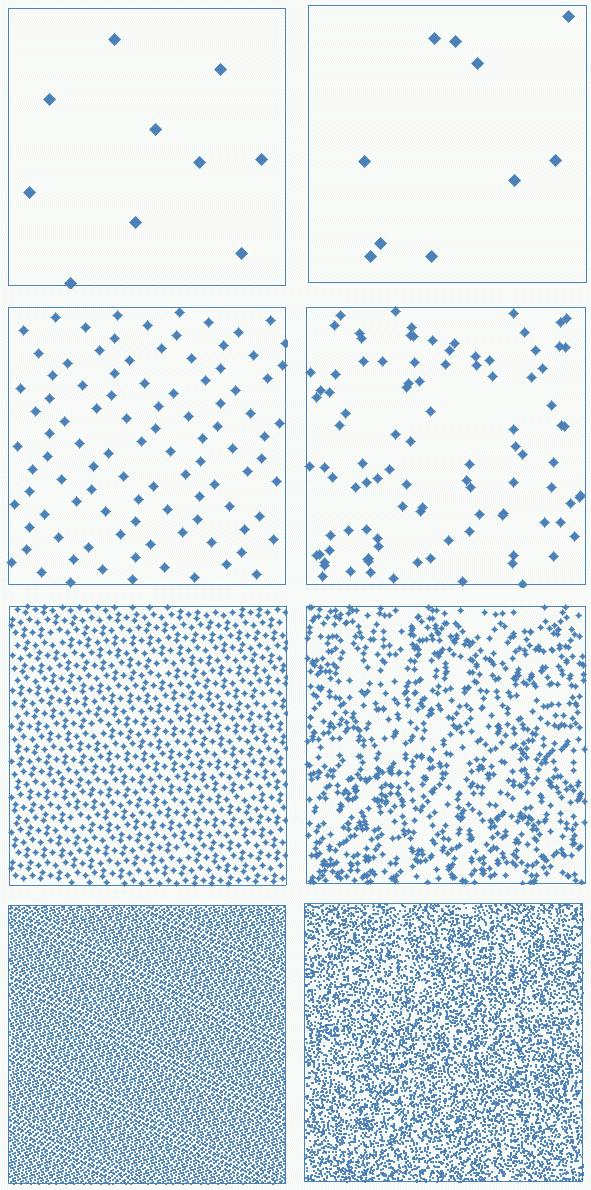
\includegraphics[height=6cm]{Subrandom_2D.png}
  \caption{Links: \textit{additive recurrent sequence}, Rechts: Zufallszahlen. Aus: \protect\url{https://en.wikipedia.org/wiki/Low-discrepancy_sequence}}
\end{figure}
Wie in der Vorlesung besprochen gibt es keinen generellen Konvergenzbeweis für das Nelder-Mead-Verfahren aber es ist wesentlich zuverlässiger
in der Vorgehensweise und der Rechenaufwand ist deutlich geringer als im Vergleich zu \lstinline[basicstyle=\ttfamily\color{black}]|Mutation-Selektion|.

\end{document}